\begin{figure}[ht]
    \centering
    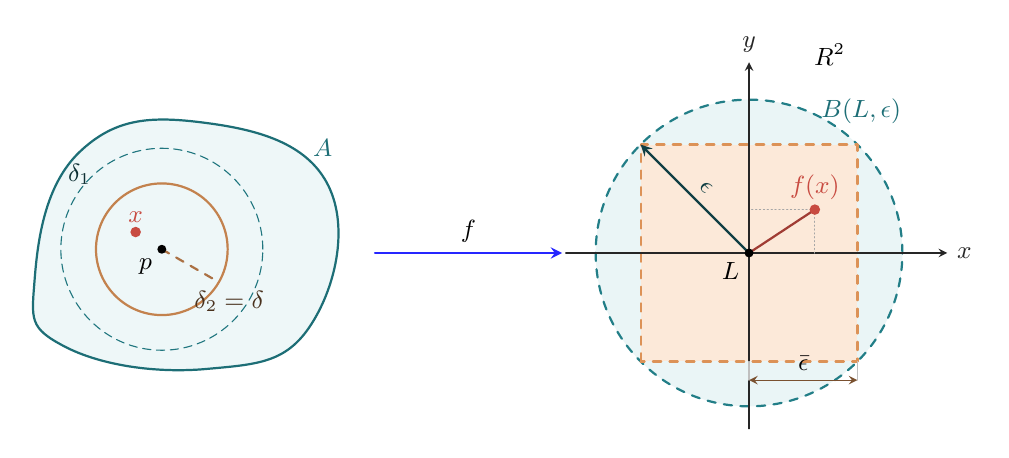
\begin{tikzpicture}[
        scale=.95,
        >=stealth,
        line cap=round,
        line join=round,
        every node/.style={font=\small}
    ]
        \definecolor{azulbola}{RGB}{42,157,169}
        \definecolor{laranja}{RGB}{244,162,97}
        \definecolor{vermelho}{RGB}{200,75,65}

        % Painel esquerdo: domínio
        \begin{scope}[xshift=-3.75cm]
            \fill[azulbola!8]
                plot[smooth cycle, tension=.75] coordinates {
                    (-2.05,-.35) (-1.45,1.35) (.15,1.75)
                    (1.85,.95) (1.65,-.95) (.25,-1.55) (-1.65,-1.25)
                };
            \draw[azulbola!70!black, thick]
                plot[smooth cycle, tension=.75] coordinates {
                    (-2.05,-.35) (-1.45,1.35) (.15,1.75)
                    (1.85,.95) (1.65,-.95) (.25,-1.55) (-1.65,-1.25)
                };

            \coordinate (p) at (-.35,.05);
            \coordinate (x) at (-.7,.28);

            \draw[azulbola!75!black, densely dashed] (p) circle (1.35);
            \draw[laranja!90!black, densely dashed] (p) circle (.88);
            \draw[laranja!80!black, thick] (p) circle (.88);
            \draw[laranja!70!black, thick, dashed]
                (p) -- node[midway, below, sloped] {} ++(330:.88);

            \fill[black] (p) circle (1.7pt) node[below left] {$p$};
            \fill[vermelho] (x) circle (2pt) node[above] {$x$};

            \node[azulbola!30!black] at (-1.45,1.05) {$\delta_1$};
            \node[laranja!30!black] at (.55,-.65) {$\delta_2=\delta$};


            \node[azulbola!70!black] at (1.80,1.40) {$A$};
        \end{scope}

        % Seta entre os painéis
        \draw[->, thick, blue!85] (-1.25,0) -- (1.25,0)
            node[midway, above, black] {$f$};

        % Painel direito: contradomínio
        \begin{scope}[xshift=3.75cm]
            \node[font=\small\bfseries, right=20pt] at (0,2.65) {$\mathbb R^2$};

            \pgfmathsetmacro{\epsrad}{2.05}
            \pgfmathsetmacro{\halfside}{\epsrad/sqrt(2)}

            \coordinate (L) at (0,0);
            \coordinate (F) at (.88,.58);
            \coordinate (Fx) at (.88,0);
            \coordinate (Fy) at (0,.58);

            \fill[azulbola!10] (L) circle (\epsrad);
            \draw[azulbola!80!black, thick, dashed] (L) circle (\epsrad);

            \fill[laranja!24]
                (-\halfside,-\halfside) rectangle (\halfside,\halfside);
            \draw[laranja!90!black, thick, dashed]
                (-\halfside,-\halfside) rectangle (\halfside,\halfside);

            \draw[->, black!85] (-2.45,0) -- (2.65,0) node[right] {$x$};
            \draw[->, black!85] (0,-2.35) -- (0,2.55) node[above] {$y$};

            \draw[azulbola!40!black, ->, thick]
                (L) -- ({\epsrad*cos(135)},{\epsrad*sin(135)})
                node[midway, above, sloped] {$\epsilon$};

            \draw[gray!50] (0,-\halfside) -- (0,-\halfside-.25);
            \draw[gray!50] (\halfside,-\halfside) -- (\halfside,-\halfside-.25);
            \draw[laranja!50!black, <->]
                (0,-\halfside-.25) -- (\halfside,-\halfside-.25)
                node[midway, above, black] {$\bar\epsilon$};

            \draw[densely dotted, gray!70] (F) -- (Fx);
            \draw[densely dotted, gray!70] (F) -- (Fy);
            \draw[vermelho!80!black, thick] (L) -- (F);

            \fill[black] (L) circle (1.7pt) node[below left] {$L$};
            \fill[vermelho] (F) circle (2pt) node[above] {$f(x)$};

            \node[azulbola!70!black] at (1.5,1.9) {$B(L,\epsilon)$};
        \end{scope}
    \end{tikzpicture}
    \label{fig:continuidadeCoord}
    \caption{À esquerda, a escolha de $\delta$ no domínio; à direita, o quadrado centrado em $L$, no caso $m=2$.}
\end{figure}
